\chapter{Research Procedure}
\label{chapter:research-proposal}

\section{Research Design}

The following chapter details the physical setup to develop the measurements that constitute the dataset under study, also present a description of testbench and processing pipeline in which the data will flow from the acoustic inputs towards the desire location-orientation output.       

\section{Methodology}

The methodology starts with the data collection under an experimental setup, the data will be curated to eliminate random noise and presented as a time series dataset. The resulting dataset will be used to train and test four neural network pipelines. The predicted location-orientation error is calculated and a multifactor Analysis of Variance (ANOVA) is proposed as the main criteria to evaluate the significant variance of the error of each processing pipeline used to estimate the location and orientation of an object in a room. 
 
\subsection{Experiment Design}
\label{section:experiment-design}
The research require the development of a manipulable and fully controllable environment in which the acoustic measurements are going to be performed. A small box type room is the volumetric cubic space proposed as the experimental container. The interior of the room needs to be easily configurable, for this a robotic arm will be allocated inside to manipulate object in the interior. An acoustic signal originated at one corner of the room will be measured and captured by microphones located in the opposite sides of the room. The figure \ref{fig:Mbox} shows the measurement setup, a six DOE robotic arm located in the center is used to move and change the position and orientation of one cube inside the box. The blue circles correspond to three microphones arrays placed in the sides of the room. One speaker positioned in the opposite angle to side in which the microphones are located is the source of the acoustic signal that will be recorded. In yellow is show the trajectory for the direct sound. The arrangement is intended to have a three axis capture composition. 

\begin{figure}[hbt!]
	\begin{center}
		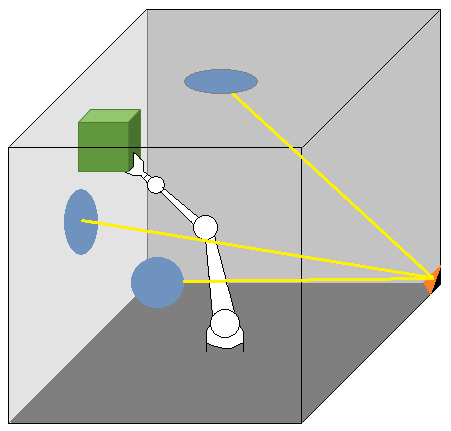
\includegraphics[width=7cm, height=7cm]{../img/Measure box.png}
		\caption{Measure box with: the robotic arm, the microphone measurement arrays and the source signal speaker.}
		\label{fig:Mbox}
	\end{center}
\end{figure}

Each microphone array is composed of four microphones placed in pairs as show in figure \ref{fig:Binaural}. A binaural horizontal pair allowed directive selection in X axis, while a binaural vertical does it in Y axis. The figure \ref{fig:method} shows the different pipelines proposed to transform the echoes measurements into coordinates. 

\begin{figure}[hbt!]
	\begin{center}
		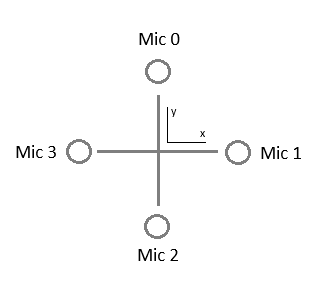
\includegraphics[width=4cm, height=4cm]{../img/BinauralPairs.png}
		\caption{Microphone array configured as binaural pairs in horizontal and vertical}
		\label{fig:Binaural}
	\end{center}
\end{figure}


\begin{figure}[hbt!]
	\begin{center}
		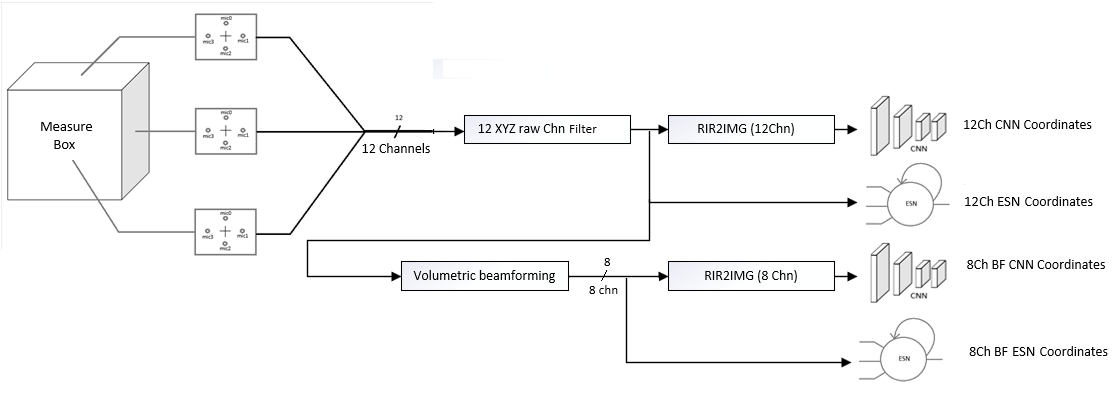
\includegraphics[width=15.5cm, height=6cm]{../img/method2.png}
		\caption{Acustic to location processing pipeline}
		\label{fig:method}
	\end{center}
\end{figure}


In figure \ref{fig:method} the three arrays together result in a twelve channel measure, this channels are used to feed the pipelines. First a filtering stage is intended to remove the noise based on the cross-spectral densities between channels [22]. The post filter twelve channels are feeding four parallel processing paths. One that use only CNN needs the time series to be transformed to images representation in order to train and evaluate the performance of a CNN as the coordinates estimator. Exist other that use ESN and due the fact that the recurrent neural network by principle can directly learn from time series, we explore the impact that have the time series to image transformation by removing this stage and train directly a RC RNN. Finally An improvement suggested to overcome the superposition problem consider the use of beamforming to create a segmented origin representation of the acoustic reverberation, with this the room space is divide in 8 different regions and the sound originated from those regions is contained in a group of new created channel that will also feed a CNN and ESN estimators.

\subsection{Factors and Levels}

For the experimental analysis, the factors and their respective levels to consider are summarized in the table \ref{tab:facandlev}. As described in previous section the microphone location will have three different arrays located in different wall of the room. The channel count is twelve. The beamforming effect is also considered. The Network is a factor as well with two proposed topologies CNN and ESN as levels.     


\begin{table}[hbt!]
	\caption{Factors and levels for the experiment.}
	\label{tab:facandlev}
	\begin{center}
		\begin{tabular}{|l|l|l|l|}
			\cline{2-4}
			\multicolumn{1}{c|}{}	& \multicolumn{3}{c|}{Factors} \\ 
			\cline{2-4}
			\multicolumn{1}{c|}{}	& Mic location - Num Channels & Beamforming & Network \\ \hline
			Levels
			& Three locations, 12 Channels	& with     & CNN  \\
			&  & without  & ESN  \\\hline
		\end{tabular}
	\end{center}
\end{table}


%\begin{table}[hbt!]
%	\caption{Factors and levels for the experiment.}
%	\label{tab:facandlev}
%	\begin{center}
%		\begin{tabular}{|l|>{\centering\arraybackslash}p{10cm}|}
%			\cline{2-2}
%			\multicolumn{1}{c|}{}	& Factors  \\ 
%			\cline{2-2}
%			\multicolumn{1}{c|}{}	& Mic location - Num Channels - Beamforming - Network \\ \hline
%			Levels
%			& Single location, 4 Channels, without, CNN  \\
%			& Three locations, 3 Channels, without, CNN  \\
%			& Three locations, 12 Channels, without, CNN \\
%           & Three locations, 12 Channels, with, CNN  \\
%            & Three locations, 12 Channels, with, ESN  \\ \hline
%		\end{tabular}
%	\end{center}
%\end{table}

The minimal amount of repetitions required by an ANOVA analysis is two, for this experiment we are going to perform 5 runs with 500 points measurements each run.  


\subsection{Response Variable}
The response variable is the error from the estimated coordinates of the XYZ location and two angular values that describe the orientation of the cube in the room. Those values are obtained from the output of the neural networks.  

%\subsection{Experiment set-up}

\subsection{Data Collection}

The data will be collected on six rounds of measurement as show in table \ref{tab:acmeasure}, a first sample of 1000 values responses correspond to train the neural networks, the other five repetitions of 500 samples are going to be use for the experiment analysis.     
For the data recollection a python script will be responsible to control the arm to move the object to a new location, trigger the acoustic swap signal and open the recording microphones channels to record the response. The start location will be randomly selected, a measure will be perform followed by a small local random increments less than 5 cm to calculate the new location. after 10 small measurements, a new full random location will be calculated and the robotic arm will be relocated to that position and a small random displacement again will be perform. This process will continue until the sample for the run is completed.        



\begin{table}[h]
	\caption{Acoustic Samples}
	\label{tab:acmeasure}
	\begin{center}
		\begin{tabular}{|l|l|l|l|l|l|l|}
            \hline
            \multicolumn{7}{|c|}{Acoustic Measurements} \\
            \hline
             & \multicolumn{6}{|c|}{Type Per Use} \\ 
            %\multicolumn{5}{|c|}{Count} \\
            \hline
			& Training  & test1 &  test2 & test3 & test4 & test5\\
            \hline
			Samples & 1000  & 500 &  500 & 500 & 500 & 500\\
            \hline
            
		\end{tabular}
	\end{center}
\end{table}


\subsection{Statistical Tool Used Description}

All the data analysis will be perform in R using the package extension for the multifactor ANOVA processing. 